\documentclass[a4paper, 12pt]{article} % тип документа

%%%Библиотеки
	%\usepackage[warn]{mathtext}	
	\usepackage[T2A]{fontenc}   %Кодировка
	\usepackage[utf8]{inputenc} %Кодировка исходного текста
	\usepackage[english, russian]{babel} %Локализация и переносы
	\usepackage{caption}
	\usepackage{gensymb}
	\usepackage{listings}
	\usepackage{amsmath, amsfonts, amssymb, amsthm, mathtools}
	\usepackage[warn]{mathtext}
	\usepackage[mathscr]{eucal}
	\usepackage{wasysym}
	\usepackage{graphicx} %Вставка картинок правильная
	\usepackage{pgfplots}
	\usepackage{indentfirst}
	\usepackage{float}    %Плавающие картинки
	\usepackage{wrapfig}  %Обтекание фигур (таблиц, картинок и прочего)
	\usepackage{fancyhdr} %Загрузим пакет
	\usepackage{lscape}
	\usepackage{xcolor}
	\usepackage[normalem]{ulem}
	
	\usepackage{titlesec}
	\titlelabel{\thetitle.\quad}

	\usepackage{hyperref}

%%%Конец библиотек

%%%Настройка ссылок
	\hypersetup
	{
		colorlinks = true,
		linkcolor  = blue,
		filecolor  = magenta,
		urlcolor   = blue
	}
%%%Конец настройки ссылок


%%%Настройка колонтитулы
	\pagestyle{fancy}
	\fancyhead{}
	\fancyhead[L]{2.5.1}
	\fancyhead[R]{Глаз Роман, группа Б01-007}
	\fancyfoot[C]{\thepage}
%%%конец настройки колонтитулы



\begin{document}
						%%%%Начало документа%%%%


%%%Начало титульника
\begin{titlepage}

	\newpage
	\begin{center}
		\normalsize Московский физико-технический институт \\(госудраственный университет)
	\end{center}

	\vspace{6em}

	\begin{center}
		\Large Лабораторная работа по общему курсу физики\\Термодинамика и молекулярная физика
	\end{center}

	\vspace{1em}

	\begin{center}
		\Large \textbf{2.5.1. Измерение поверхностного натяжения жидкости }
	\end{center}

	\vspace{2em}

	\begin{center}
		\large Глаз Роман Сергеевич\\
		Группа Б01-007
	\end{center}

	\vspace{\fill}

	\begin{center}
		Долгопрудный \\2021
	\end{center}
	
\end{titlepage}
%%%Конец Титульника



%%%Настройка оглавления и нумерации страниц
	\thispagestyle{empty}
	\newpage
	\tableofcontents
	\newpage
	\setcounter{page}{1}
%%%Настройка оглавления и нумерации страниц


					%%%%%%Начало работы с текстом%%%%%%

\textbf{Цель работы:} 1) измерение температурной зависимости коэффициента поверхностного натяжения дистиллированной воды с использованием известного коэффициента поверхностного натяжения спирта; 2) определение полной поверхностной энергии и теплоты, необходимой для изотермического образования единицы поверхности жидкости при различной температуре.\\

\textbf{Используемое оборудование:} прибор Ребиндера с термостатом и микроманометром; исследуемые жидкости; стаканы.

\section{Теоретические сведения}

Поверхностное натяжение имеет двойной физический смысл -- энергетический (термодинамический) и силовой (механический). Энергетическое (термодинамическое) определение: поверхностное натяжение -- это удельная работа увеличения поверхности при её растяжении при условии постоянства температуры. Силовое (механическое) определение: поверхностное натяжение -- это сила, действующая на единицу длины линии, которая ограничивает поверхность жидкости

Наличие поверхностного слоя приводит к различию давлений по разные стороны от искривленной границы раздела двух сред. Для сферического пузырька с воздухом внутри жидкости избыточное давление даётся формулой Лапласа:

\begin{equation}
\Delta P = P_{inside} - P_{outside} = \frac{2\sigma}{r},
\label{eq:1}
\end{equation}

где $\sigma$ – коэффициент поверхностного натяжения, $P_{inside}$ и $P_{outside}$ – давление внутри пузырька и снаружи, $r$ – радиус кривизны поверхности раздела двух фаз. Эта формула лежит в основе предлагаемого метода определения коэффициента поверхностного натяжения жидкости. Измеряется давление $\Delta P$, необходимое для выталкивания в жидкость пузырька воздуха.

\section{Экспериментальная установка}

Исследуемая жидкость (дистиллированная вода) наливается в сосуд (колбу) $B$. Тестовая жидкость (этиловый спирт) наливается в сосуд $E$. При измерениях колбы герметично закрываются пробками. Через одну из двух пробок проходит полая металлическая игла $C$. Этой пробкой закрывается сосуд, в котором проводятся измерения. Верхний конец иглы открыт в атмосферу, а нижний погружен в жидкость. Другой сосуд герметично закрывается второй пробкой. При создании достаточного разряжения воздуха в колбе с иглой пузырьки воздуха начинают пробулькивать через жидкость. Поверхностное натяжение можно определить по величине разряжения $\Delta P$ (\ref{eq:1}), необходимого для прохождения пузырьков (при известном радиусе иглы).

\bigskip

Разряжение в системе создается с помощью аспиратора $A$. Кран К$_2$ разделяет две полости аспиратора. Верхняя полость при закрытом кране К$_2$ заполняется водой. Затем кран К$_2$ открывают и заполняют водой нижнюю полость аспиратора. Разряжение воздуха создается в нижней полости при открывании крана К$_1$, когда вода вытекает из неё по каплям. В колбах $B$ и $C$, соединённых трубками с нижней полостью аспиратора, создается такое же пониженное давление. Разность давлений в полостях с разряженным воздухом и атмосферой измеряется спиртовым микроманометром (устройство микроманометра описано в Приложении).
Для стабилизации температуры исследуемой жидкости через рубашку $D$ колбы $B$ непрерывно прогоняется вода из термостата.

\begin{figure}[h]
    \centering
    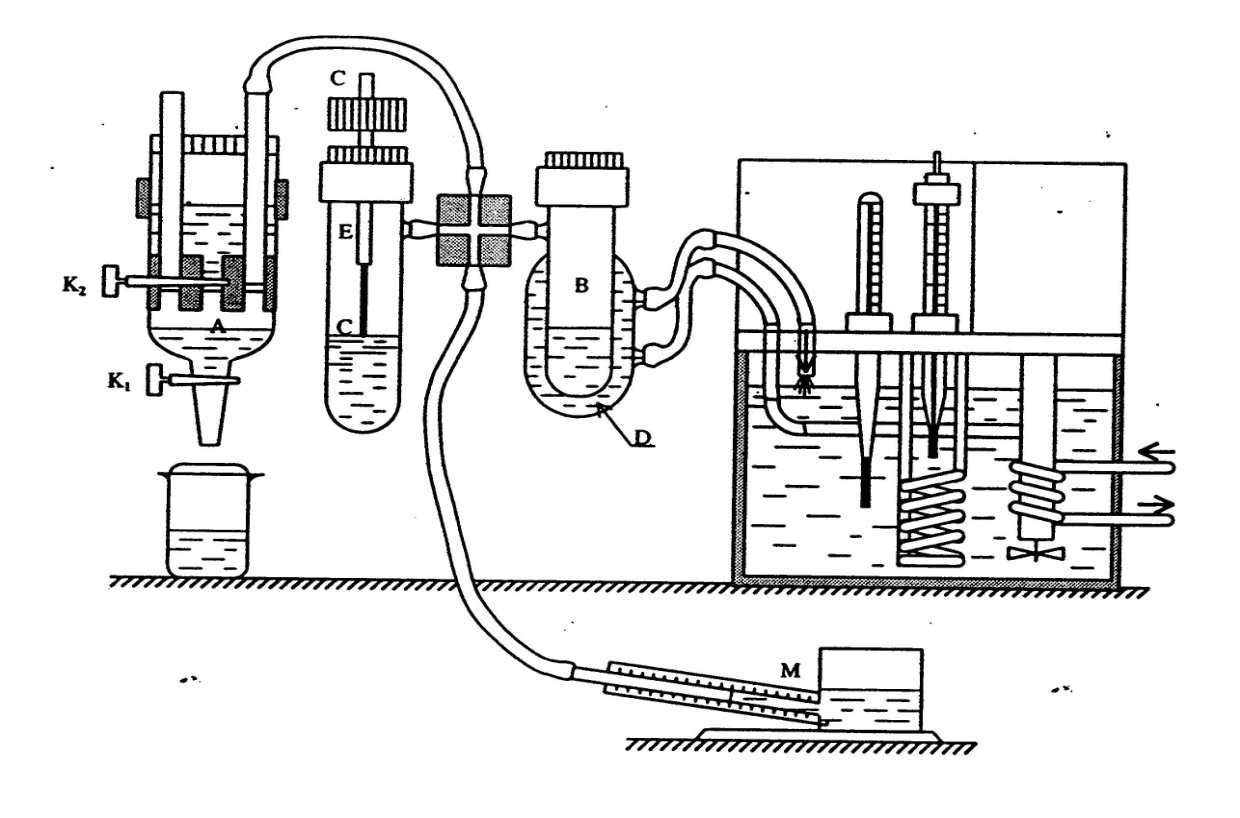
\includegraphics[width=1\textwidth]{Scheme.jpg}
    \caption{Схема установки для измерения поверхностного натяжения}
    \label{fig:vac}
\end{figure}


Обычно кончик иглы лишь касается поверхности жидкости, чтобы исключить влияние гидростатического давления столба жидкости. Однако при измерении температурной зависимости коэффициента поверхностного натяжения возникает ряд сложностей. Во-первых, большая теплопроводность металлической трубки приводит к тому, что температура на конце трубки заметно ниже, чем в глубине жидкости. Во-вторых, тепловое расширение поднимает уровень жидкости при увеличении температуры.

Обе погрешности можно устранить, погрузив кончик трубки до самого дна. Полное давление, измеренное при этом микроманометром, $P = \Delta P + \rho gh$. Заметим, что $\rho gh$ от температуры практически не зависит, так как подъём уровня жидкости компенсируется уменьшением её плотности (произведение $\rho h$ определяется массой всей жидкости и поэтому постоянно). Величину $\rho gh$ следует измерить двумя способами. 

Во-первых, замерить величину $P1 = \Delta P'$, когда кончик трубки только касается поверхности жидкости. Затем при этой же температуре опустить иглу до дна и замерить $P_2 = \rho gh + \Delta P"$ ($\Delta P' ,\: \Delta P"$ – давление Лапласа). Из-за несжимаемости жидкости можно положить $\Delta P' = \Delta P"$ и тогда $\rho gh = P_2 -P_1$. Во-вторых, при измерениях $Р_1$ и $Р_2$ замерить линейкой глубину погружения иглы $h$. Это можно сделать, замеряя расстояние между верхним концом иглы и любой неподвижной частью прибора при положении иглы на поверхности и в глубине колбы.

\section{Измерения}

Проведем измерения для спирта. Для этого установим частоту падения капель из аспиратора около 1 капли в 5 секунд. Измерим максимальное добавочное давление в системе. Полученный результат $\Delta p = 42 \pm 1 \Rightarrow \Delta P = 81 \pm 2$ Па ($p$ -- единица длины на микробарометре, а $P$ уже искомое давление).

\bigskip

Далее вынем иглу, просушим ее и измерим микроскопом ее диаметр (внутренний):

\begin{equation}
	d = 1.2 \pm 0.05 \text{ мм},
\label{eq:2}
\end{equation}

из табличного значения коэффициента поверхностного натяжения спирта $\sigma = 22.3 \text{ мН/м}$, теперь по формуле (\ref{eq:1}) получим:

\begin{equation}
	r = \frac{2\sigma}{\Delta P} = 0,643 \text{ мм}
\end{equation}

\begin{equation}
	\Delta r = 0,015 \text{ мм}
\end{equation}

Как можно увидить экспериментальный результат совпал с прямым измерение с учётом погрешностей, что говорит о применимости нашей модели.

\bigskip

Затем установим иглу в воду так, чтобы она едва касалась воды. Измерим значение давления. Далее опустим иглу до дна, предварительно измерив высоту. Получим значение разности высот, измеренных линейкой:

\begin{equation}
	h_1 =20 \pm 1 \text{ мм; } \\ h_2 =6 \pm 1 \text{ мм}\\ \Rightarrow \Delta h = 14 \pm 2 \text{ мм.}
\label{eq:4}
\end{equation}

Теперь посчитаем разность высот из измеренных давлений: $\Delta P = 122 \pm 1,5$ Па, откуда $h = 12,4 \pm 0,2$ мм. Видно, что значение получилось немного меньше, чем измеренное линейкой, но в пределеах погрешности значения совпадают.

\begin{center}
	\begin{tabular}{|c|c|c|}
	\hline 
	№ & $ \langle h_1 \rangle, \text{ мм}$ & $\langle h_2 \rangle, \text{ мм}$ \\ 
	\hline 
	1 & 112 & 187 \\ 
	\hline 
	2 & 112 & 187 \\ 
	\hline 
	3 & 111 & 186 \\ 
	\hline 
	4 & 111 & 186 \\ 
	\hline 
	5 & 111 & 186 \\ 
	\hline
	$ \langle h \rangle$, мм & 111 & 187 \\ 
	\hline
	$ \langle P \rangle$, Па & 177 & 299 \\ 
	\hline 
	\end{tabular} 
\end{center}

\bigskip

Проведем серию измерений разности давлений $\Delta P$ для различных температур воды в интервале [20--60] $^\circ C$ (шаг $\simeq 5^\circ C$), регулируемых термостатом, занесем результаты в таблице ниже

\begin{center}
\begin{tabular}{|c|c|c|c|c|c|c|c|c|}
\hline
	$t$, $\degree C$ & $20,5$ & $25$ & $30$ & $35$ & $40$ & $45$ & $50,6$ & $55$ 	\\
	\hline
	$h$, мм & 132 & 131 & 130 & 129 & 128 & 127 & 125 & 124\\
	\hline
	$h$, мм & 132 & 131 & 130 & 129 & 127 & 126 & 125 & 124\\
	\hline
	$h$, мм & 132 & 131 & 130 & 128 & 127 & 126 & 125 & 124\\
	\hline
	$h$, мм & 132 & 130 & 129 & 128 & 127 & 126 & 125 & 124\\
	\hline
	$h$, мм & 131 & 130 & 129 & 128 & 127 & 126 & 125 & 123\\
	\hline
	$ \langle h \rangle$, мм & 131,8 & 130,6 & 129,6 & 128,4 & 127,2 & 126,2 & 125 & 123,8\\
	\hline
	$\Delta h $, мм & 1,2 & 1,28 & 1,34 & 1,4 & 1,2 & 1,2 & 1 & 1,2\\
	\hline
	$\langle P \rangle$, Па & 210,7 & 208,8 & 207,23 & 205,31 & 203,40 & 201,80 & 199,88 & 196,96 \\
	\hline
	$\Delta P$, Па & 1,93 & 2,06 & 2,16 & 2,26 & 1,93 & 1,93 & 2,06 & 1,93 \\
	\hline
\end{tabular}
\end{center}

По полученным данным можно вычислить значение $\sigma = \frac{p \cdot R}{2}$

\begin{center}
\begin{tabular}{|c|c|c|c|c|c|c|c|c|}
\hline
	$t$, $\degree C$ & $20,5$ & $25$ & $30$ & $35$ & $40$ & $45$ & $50,6$ & $55$ 	\\
	\hline
	$<P>$ & 210,7 & 208,8 & 207,23 & 205,31 & 203,40 & 201,80 & 199,88 & 196,96 \\
	\hline
	$\Delta P$, Па & 1,93 & 2,06 & 2,16 & 2,26 & 1,93 & 1,93 & 2,06 & 1,93 \\
	\hline
	$\sigma \cdot 10^2$, Н/м & 6,77 & 6,71 & 6,66 & 6,60 & 6,54 & 6,48 & 6,42 & 6,36 \\
	\hline
	$\Delta \sigma \cdot 10^2$, Н/м & 0,154 & 0,164 & 0,171 & 0,181 & 0,154 & 0,154 & 0,164 & 0,154 \\
	\hline
\end{tabular}
\end{center}

При подсчёте погрешностей поверхностного наяжения были учетны погрешности определения радиуса иглы.


\bigskip

\section{Обработка данных}

\smallskip

Построим график зависимости $\sigma(T)$

\smallskip

Из графика \textit{методом хи-квадрат} найдем коэффициент наклона:

\smallskip

\begin{equation}
	\frac{d \sigma}{dT} = -0.137 \text{ мН} \cdot \text{м} / K
\end{equation}


\begin{equation}
	\Delta \frac{d \sigma}{dT} = 0,0067 \text{ мН} \cdot \text{м} / K
\end{equation}

Сравним с табличным:

\begin{equation}
	\frac{d\sigma_t}{dT} = -0.154\ \text{мН} \cdot \text{м} / K
\end{equation}

В целом значения сходятся, однако теоретическое значение вышло больше, чем полученное экспериментальное.

\begin{figure}[h]
	\center{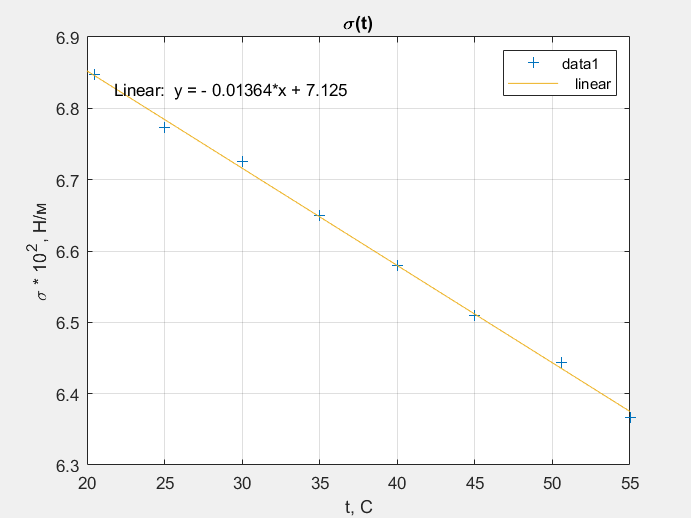
\includegraphics[scale = 0.7]{graph1.png}}
	\caption{Зависимость коэффициента поверхностного натяжения от температуры}
	\label{gr:1}
\end{figure}

Теперь, зная все нужные значения, построим графики зависимостей $q(t) = -T \frac{d \sigma}{dT}$ и $\frac{U}{F}(T) = \sigma - T\frac{d \sigma}{dT}$. Видно, что в последнем графике значение поверхностной энергии на единицу площади почти не меняется.

\begin{figure}[h]
	\center{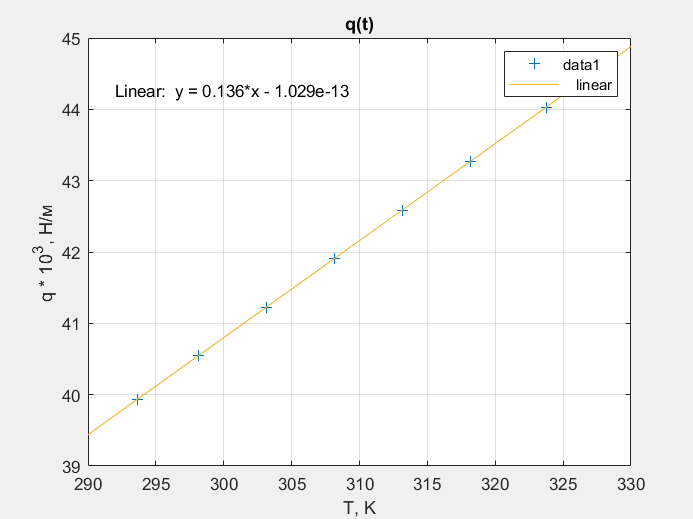
\includegraphics[scale = 0.7]{graph2.png}}
	%\caption{Сферическая система координат наглядно}
	\label{gr:2}
\end{figure}

\begin{figure}[h]
	\center{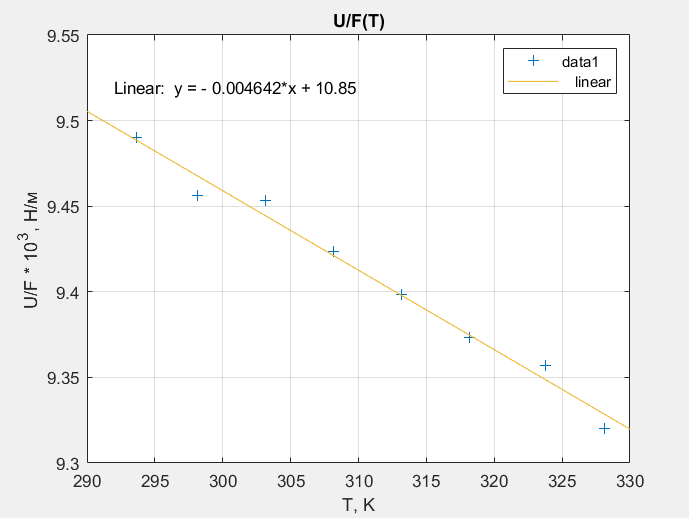
\includegraphics[scale = 0.7]{graph3.png}}
	%\caption{Сферическая система координат наглядно}
	\label{gr:3}
\end{figure}


\section{Заключение}

В работе эксперементально был измерен коэффициент поверхностного натяжения воды, с учетом известного коэффициента поверхностого натяжения спирта. Полученное значение совпадает с табличным по порядку величины, но не совпадает в пределах погрешности. Сильное влияние могло оказать низкая точность поправочного давления на глубине сосуда, неидеальность иглы.

Во чторой части была экспериментально установлена линейная зависимость коэффициента поверхностного натяжения от температуры.

\section{Список используемой литературы}

$\bullet$ Гладун А. Д. Лабораторный практикум по общей физике. Термодинамика и молекулярная физика\\

$\bullet$ \href{https://mipt.ru/education/chair/physics/S_II/lab/}{Описание лабораторных работ на кафедре общей физики МФТИ}

\end{document}